\documentclass[UTF8]{scrartcl}

\usepackage{xeCJK}
\usepackage{graphicx}
\usepackage{subfigure}
\usepackage{indentfirst}
\setlength{\parindent}{2em}

%opening
\title{算法\&架构整理v1.0}
\author{Fan Yinghui}

\begin{document}

\maketitle

\begin{abstract}

\end{abstract}

\section{硬件架构}

 图一给出了卷积(Convolution)计算的伪代码、示意图和典型的加速器架构图。从伪代码中可以看出卷积计算有6个循环,基本计算为乘加计算,循环体中计算的索引小标则反映了循环间的数据复用和数据依赖。典型的加速器架构包括global buffer(一般几百KB,与DRAM相连)、PE阵列(PE之间有一定互联关系)、每个PE中还有Registor File(RF一般几KB或更小)。

	\begin{figure}[h]
		\centering
		\subfigure[卷积伪代码]{ 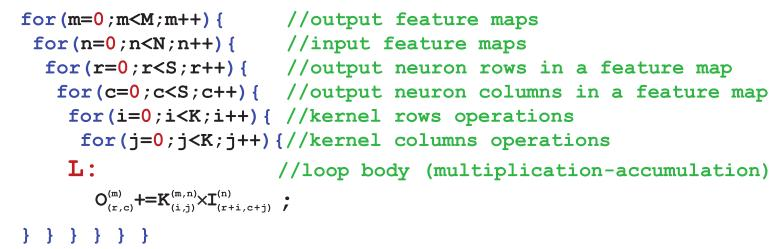
\includegraphics[width=2.50in,height=1.00in]{fig1.jpg} }
		\subfigure[卷积图示]{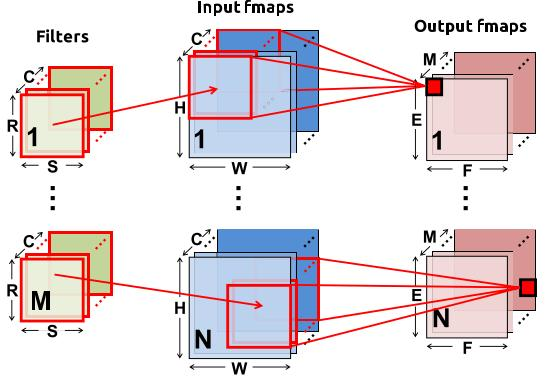
\includegraphics[width=1.50in, height=1.00in]{conv_graph.jpg}}
		\subfigure[加速器图示]{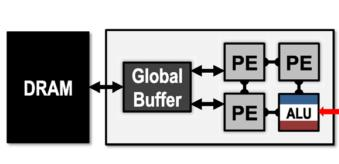
\includegraphics[width=1.50in, height=1.00in]{acc.jpg}}
		\caption{卷积计算及硬件架构}
		\label{fig1}
	\end{figure}
	

 加速器设计首先要考虑的问题即设计合适的dataflow将卷积计算映射到PE阵列和存储层次中,有两个考虑的角度,一是充分利用计算中的数据复用,减少可复用数据的访存次数,由此降低功耗; 二是充分利用计算中的可并行性,选择合适的循环展开方法,增大吞吐量。

	 \subsection{数据复用}
	 加速器的存储结构包括PE单元内部的RF、片内的Global Buffer以及片外DRAM,从不同的存储单元中读取数据所消耗的能量不同。而卷积的计算中提供了三种数据复用的可能:1. convolution reuse; 2. featuremap reuse; 3.filter reuse。
	 
	%	\begin{figure}[h]
	% 		\centering
	 %		 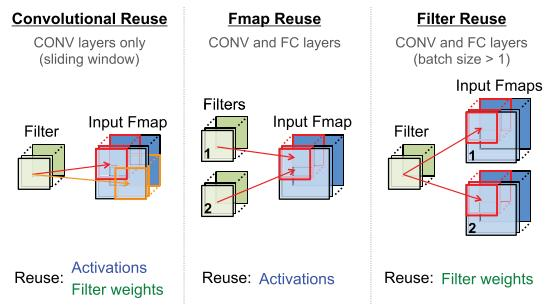
\includegraphics[width=5.50in,height=3.00in]{reuse.jpg} 
	 %		\caption{卷积计算中的数据复用}
	 %		\label{fig2}
	 %	\end{figure}
	 
	 因此从数据复用角度看,尽可能将可复用的数据存在local Memory中,减少从DRAM中读取的次数,则可以降低功耗。根据将何种数据存在local mem中,dataflow可以分为以下几种\cite{sze2017efficient}:
		 \subsubsection{Weight Stationary}
		 将不同的权重存在RF中,并尽可能多的利用这些权重进行计算。因此每个PE的RF存储不同的权重,同一激活层数据广播至所有的PE单元,而同一个Psum通过每一个PE单元并累加获得最终结果。代表案例是NeuFlow\cite{neoflow}。
		 \subsubsection{Output Stationary}
		 将中间和Patial Sum存在RF中,减少从buffer和DRAM中读取Psum的次数。因此Psum存在RF中不动,将同一权重广播至所有PE单元,而同一个Act依次通过每一个PE单元。Psum可以来自同一通道不同位置、不同通道同一位置或不同通道不同位置。代表案例是ShiDianNao\cite{du2015shidiannao}。
		 
		 	\begin{figure}[h]
		 		\centering
		 		\subfigure[WS]{ 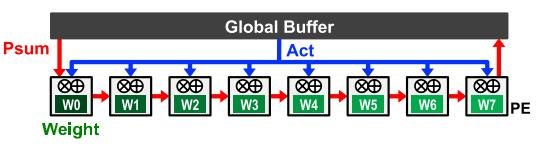
\includegraphics[width=2.60in,height=1.00in]{ws.jpg} }
		 		\subfigure[OS]{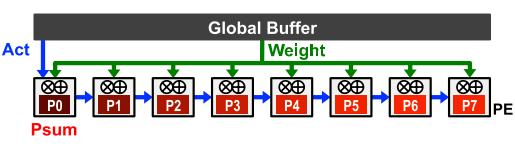
\includegraphics[width=2.60in, height=1.00in]{os.jpg}}
		 		\subfigure[NLR]{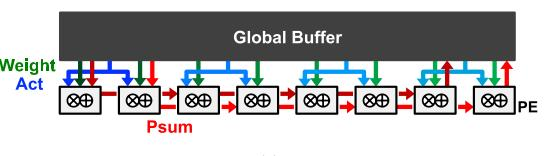
\includegraphics[width=2.60in, height=1.00in]{nlr.jpg}}
		 		\subfigure[RS]{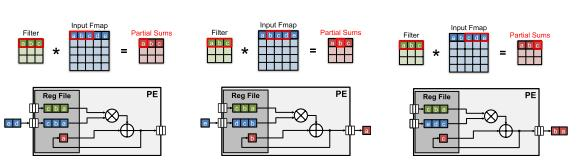
\includegraphics[width=2.70in, height=1.00in]{rs.jpg}}
		 		\caption{Dataflow}
		 		\label{fig2}
		 	\end{figure}
		 
		 
		 \subsubsection{No Local Reuse}
		 不再使用local的RF,全部使用global buffer,减少与DRAM的数据交换。因此通过复制多份Act,与权重计算,并通过累加各个PE的Psum获得最终结果。代表案例是DianNao\cite{diannao}和DaDianNao\cite{dadiannao}。
		 \subsubsection{Row Stationary}
		 针对所有类型的数据(w,act , psum)最大化RF Level的数据复用,其计算方法如Figure2(d)。代表案例是Eyeriss\cite{eyeriss}。
	
	  \subsection{循环展开}
		  加速器的设计中一般通过将循环展开并行化的方式来实现加速,卷积计算共有6个循环可以展开,根据循环展开的策略,卷积计算中的并行度分为3类,Feature map Parallelism(FP,对应循环m,n),Neuron Parallelism (NP,对应循环r,c),Synapse Parallelism (SP,对应循环i,j),考虑是否支持这3种并行度,共有8种相应的dataflow。目前大部分加速器设计是其中的三种dataflow,对应的架构依次是Systolic、Tile-based和2D-Mappling。
		  

		  
		  \subsubsection{SFSNMS}
		  按kernel的index展开,SFSNMS,每次取一个input,broadcast至所有的PE,每个PE取一个权重(3x3 kernel),计算结果为9个对应位置的部分和。每个cycle部分和向下一个PE移动或进入队列或下一行,完成后最终输出output某一位置的结果。数据复用:相邻位置的output被mapping到不用的PE中,空间上复用了同一个输入,时间上通过每个PE的寄存器复用了权重数据。代表架构(systolic):Neuflow\cite{neoflow}。
		  
		  		  \begin{figure}[h]
		  		  	\centering
		  		  	\subfigure[Loop Unroll]{ 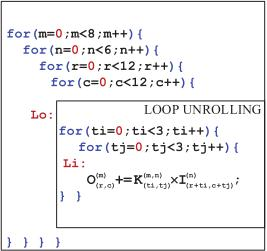
\includegraphics[width=1.5in,height=1.50in]{sfsnms.jpg} }
		  		  	\subfigure[Dataflow]{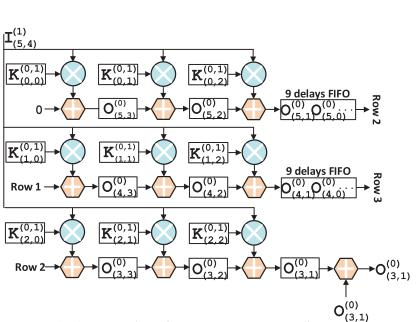
\includegraphics[width=1.5in, height=1.50in]{d1.jpg}}
		  		  	\caption{SFSNMS}
		  		  	\label{fig3}
		  		  \end{figure}
		  
		  \subsubsection{SFMNSS}
		  按照output的位置索引展开,一次计算多个output位置的结果。然后输入多个位置的input和同一个权重,输出多个位置output。从右向左从上向下传递累加,最终输出。数据复用:相邻位置的output被mapping到不同的PE中,空间上复用了同一个权重,通过PE的连接和寄存器时间上复用了input。代表架构(2D-Mapping):ShiDianNao\cite{shidiannao}。
		  
		  		 \begin{figure}[h]
		  		  		  	\centering
		  		  		  	\subfigure[Loop Unroll]{ 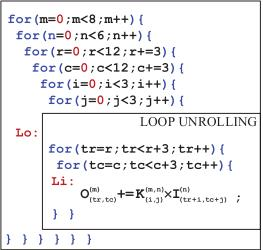
\includegraphics[width=1.5in,height=1.50in]{sfmnss.jpg} }
		  		  		  	\subfigure[Dataflow]{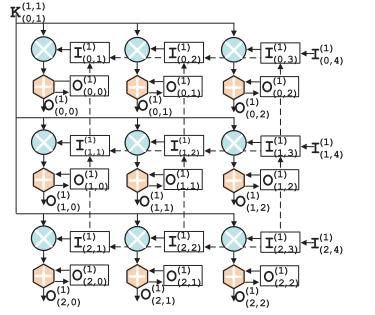
\includegraphics[width=1.5in, height=1.50in]{d2.jpg}}
		  		  		  	\caption{SFMNSS}
		  		  		  	\label{fig4}
		  		  \end{figure}		  
		  
		  \subsubsection{MFSNSS}
	      按照通道索引展开,输入同一位置不同通道的input和不同通道不同kernel(对应output的维度)的权重,输出同一位置不同通道的output。数据复用:不同的PE空间上复用了同一个input,但无法在空间上复用权重和output,这种计算架构数据复用最小。代表架构(tiling):DianNao\cite{diannap}、DaDianNao\cite{dadiannao}。
	      
	      		  		  \begin{figure}[h]
	      		  		  	\centering
	      		  		  	\subfigure[Loop Unroll]{ 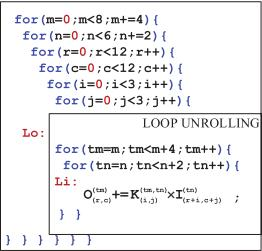
\includegraphics[width=1.5in,height=1.50in]{mfsnss.jpg} }
	      		  		  	\subfigure[Dataflow]{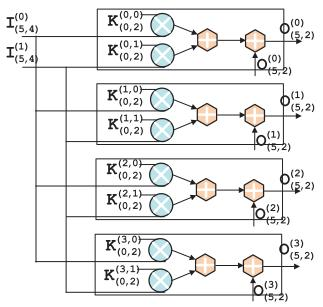
\includegraphics[width=1.5in, height=1.50in]{d3.jpg}}
	      		  		  	\caption{MFSNSS}
	      		  		  	\label{fig5}
	      		  		  \end{figure}
	      
	      
	  \subsection{总结分析}
		  %\begin{itemize}
			%  \item
			%  \item	 
			  			  
	      % \end{itemize}
		数据复用与循环展开是对卷积计算分析的两个角度,两者之间存在着一定的对应关系。数据复用可以看作将input、output或weight之一的index展开,反映在硬件上即是这些数据存在local mem中不动,可调整的index则体现了循环展开的可能性。以Neoflow为例,按照数据复用分类其属于权重复用,每个PE存一个不同的权重并尽可能多地利用这个权重进行计算,权重的不同体现在索引 \{i,j\} 的不同,对应循环展开即是SFSNMS。
		
		实际加速器设计中,dataflow可以是这些分类的组合或变种,其形式更为灵活\cite{flexflow}; 此外,dataflow与硬件架构也不是严格的一一对应,例如Diannao和 kernel partitia\cite{c-brain}l。
		
		这两个分类方法为分析加速器的Dataflow和架构设计提供了非常好的参考,一般的设计其数据复用和循环展开都会落在这样的分类下。不过能否从分类正向推导或排列组合出所有可能的形式?要考虑的问题太多还想不清楚。

	   
	 
	  \subsection{与Aladdin对比}
       Aladdin建模的硬件对象主要是存储和控制部分,不包括控制逻辑。其中存储包括ScrarchPad(buffer)和Register,可调整的参数为存储资源大小、数据排布方式、带宽、位宽等。计算部分则是并行的PE阵列(Datapath)组成,可调整的设计参数为并行度和流水线。
       
       %Aladdin的Loop Unrolling机制,展开后计算之间要无数据依赖。
       
       Aladdin的loop unrolling体现了负载应用在硬件中并行执行的情况,但无法体现这些并行单元之间的信息交互。1.1中的数据复用是指在RF这个层次的复用,要求数据能在不同的PE间传输,Aladdin的目前建模方法显然无法满足,只能支持no local reuse这一类型,即不需要PE内的RF,其数据复用体现在global buffer这个层次。而从循环展开的角度看也是这样,Aladdin要求展开循环的计算不能有PE间交互的需求。
       
        综上所述,Aladdin目前所能建模的硬件架构典型结构是 Tile-based,可行的循环展开方式有?。
  
  \section{量化算法}
  
	  \subsection{算法分类}
	  考虑CNN量化后对硬件设计的影响,将量化算法分为两类:一是近改变计算位宽不需要改变计算单元类型,代表案例是Dorefa-Net; 二是需要新的计算单元设计,例如BNN、logNet等。
	  
	  \subsection{实验分析与数据统计}
	   算法部分以Cifar10 (cifar100)为测试数据集,参考AlexNet设计相应的网络架构,需要注意:Baseline精度是否足够、网络结构复杂度是否足够(参考硬件设计中测试用的网络结构)。在数据集和网络架构固定的情况下,进行不同量化算法的对比实验,除了统计模型精度外,还应计算的参数如下:
	   
	   \begin{table}[h]
	   	\centering
	   	\caption{统计数据}
	   	\begin{tabular*}{8cm}{c |c| c |c }
	   		\hline
	   	       & 精度  &  MAC总数  & Mem占用   \\
	   	     \hline
	   	     网络层& & &\\
	   	     \hline
	   	     量化算法& & &\\
	   	     \hline
	   	     位宽& & &\\
	   	    \hline
	   		
	   		
	   	\end{tabular*}	
	   \end{table}
	   
	    \begin{table}[h]
	    	\centering
	    	\caption{网络架构参数}
	    	\begin{tabular*}{8cm}{c |c|  }
	    		\hline
	    		& XXNet       \\
	    		\hline
	    	     Input Size& \\
	    		\hline
	    		Num of Conv Layers & \\
	    		\hline
	    	   Num of FC Layers& \\
	    	    \hline
	    	    Num of Channels & \\
	    	    \hline
	    	    Num of Filters & \\
	    		\hline
	    		
	    		
	    	\end{tabular*}	
	    \end{table}
  
  \section{针对量化的计算单元和存储调整}
	  量化算法应用于卷积神经网络后,数值精度改变进而改变表示数据所需的位宽,反映在硬件上主要包扩计算和存储两大类问题,即数据表示所需的位宽与硬件计算 、存储的位宽之间不匹配,下面分别讨论。
	  \subsection{计算}
	  1) one-size-fits-all:在数据位宽小于等于计算位宽情况下,用相同的最大所需配置执行所有计算,代表案例DianNao\cite{diannao}。
	  
	  2) operand narrowing:窄位宽的数据通过宽的计算单元时,低位为0,晶体管开关活性降低,以此降低功耗。这样设计的好处是复杂度低,不需要做太多适配与调整,但存在资源的浪费。代表案例envision\cite{envision}。
	  
	  3) operator narrowing:另外一种情况是宽数据通过窄计算单元,如下图c所示。通过时间上复用来实现wide操作数的计算,但增加了latency。此外,有一些overhead例如额外的寄存器处理分时复用的中间存储,适合用在SIMD中增加并行度。代表案例stripe\cite{stripes}。
	  
	  4) special case:在某些特殊量化情况下,原有的乘加计算会退化为更简单的逻辑,于是可以使用更简单的计算单元。代表案例BNN\cite{finn}, Shifter-based\cite{shift}。
	  
	  \subsection{访存}
	  
	  1) Fixed-length:当数据位宽发生改变,依然可以用统一的存储位宽,低位置零不使用即可,设计复杂度低,但不能有效节省存储空间。
	  
	  2) Data Packing and Unpacking。将不同数据宽度的data打包到fixed-length的存储空间中,减少了带宽和存储的需求,但增加了访问数据的复杂度。这里也分两个层次,当数位宽度是2的指数时,恰好可以pack在32bit存储里;而当数位宽度更灵活,如7,9等,即便pack在32bit数里,也存在数位对齐的问题。代表案例proteus\cite{proteus}。
	  
	    
  \section{总结}
  结合总结,将涉及到的从算法到硬件的设计空间列表整理如下。
   \begin{table}[h]
	   	\centering
	   	\caption{设计空间汇总}
	   	\begin{tabular*}{16cm}{c |c| c |c }
	   		\hline
		   		Level & Space & ..  & Implementation\\
		   	\hline
			   	Arch  & Tile-Based & Tm,Tn,Buffer Size, MemPorts &  Configure\\
		   	\hline
			   	Data flow & MFSNSS &  &C code\\
		   	\hline
			   	Quantization & Float & 32bit & Pytroch\\
			   	& Fixed point & 2,4,8,16 bit&\\
			   	& Power of 2 & 2,4,8,16 bit&\\
			   	& Binary & 1 bit&\\
		   	\hline
			   	Compute Unit & float mult &与算法对应& PPA model \\
				& fixed mult & bit-parallel bit-serial & based on RTL\\
				& Shifter &&\\
				& Xnor &&\\
			 \hline
				 Mem Access & Pack \& Unpack &Buffer Size, MemPorts&添加Node ,C Code\\
			\hline
		   	
		   			   	
	   	\end{tabular*}
   \end{table}


\bibliographystyle{plain}

\bibliography{refer}


\end{document}
